\chapter{面向DSP的嵌入式微处理器设计与实现}

本章节对本文所实现的基于RISC-V的面向DSP的嵌入式微处理器进行介绍。本文所实现的微处理器主要应用场景为物联网设备、移动终端等需要满足低功耗前提,同时具有一定计算能力的设备。本文所实现的微处理器具有以下的特性:

\begin{enumerate}
	\item 实现了RISC-V中的RV32GCP指令集,即实现了32位整数指令集“I”、乘除指令集“M”、原子操作指令集“A”、单精度浮点指令集“F”、双精度浮点指令集“D”、压缩指令集“C”以及专为DSP运算增强的SIMD指令集“P”[40]。
	\item 微处理器的流水线基本框架参考了CV32E40P开源微处理器的实现,微处理器流水线采用单发射顺序执行4级流水线设计,4个流水级分别为取指(IF)、译码(ID)、执行(EX)以及写回(WB)。除了加载指令以及需要写回寄存器组的指令外,都在执行阶段完成并提交。对于存储器相关指令,则提交给加载存储单元(Load Store Unit,LSU)执行,LSU通过核内自定义的总线协议与缓存交互。
	\item 微处理器中“P”指令集采用了并行多数据通路的策略实现,通过扩展译码器以及ALU的方式实现SIMD相关指令。微处理器软核IP中可以根据实际应用需要,通过配置不同的参数生成带有“P”指令集扩展的RTL代码或仅支持RV32GC基本实现的RTL代码。
	\item 微处理器核仅实现了机器模式的特权级架构,并实现了核内本地中断控制器CLINT(Core Local Interrupt Controller)以提供带优先级的可抢占式中断服务。
	\item 微处理器外围适配的SoC片上系统实现了RISC-V Debug调试模块以及串口、GPIO、I2C、SPI等外部总线,片上总线使用AMBA AXI4总线协议,对于低速的外设,则使用低功耗的APB总线协议。APB与AXI4之间协议通信通过APB桥进行转换。
\end{enumerate}

微处理器RTL级描述完全通过PyHCL实现并验证,并通过riscv-tests[41]测试。以该微处理器为内核的SoC片上系统在Xilinx N4 FPGA平台上成功部署并进行CoreMark[42]性能测试。本章节将从以下四个方面对微处理器的实现进行介绍:流水线具体实现、特权模式实现、“P”指令集实现以及SoC片上系统实现。在本章节的最后给出微处理器的相关测试数据。图3-1给出包含该微处理器内核的SoC片上系统的概览。

\begin{figure}[htbp]
	\centering
	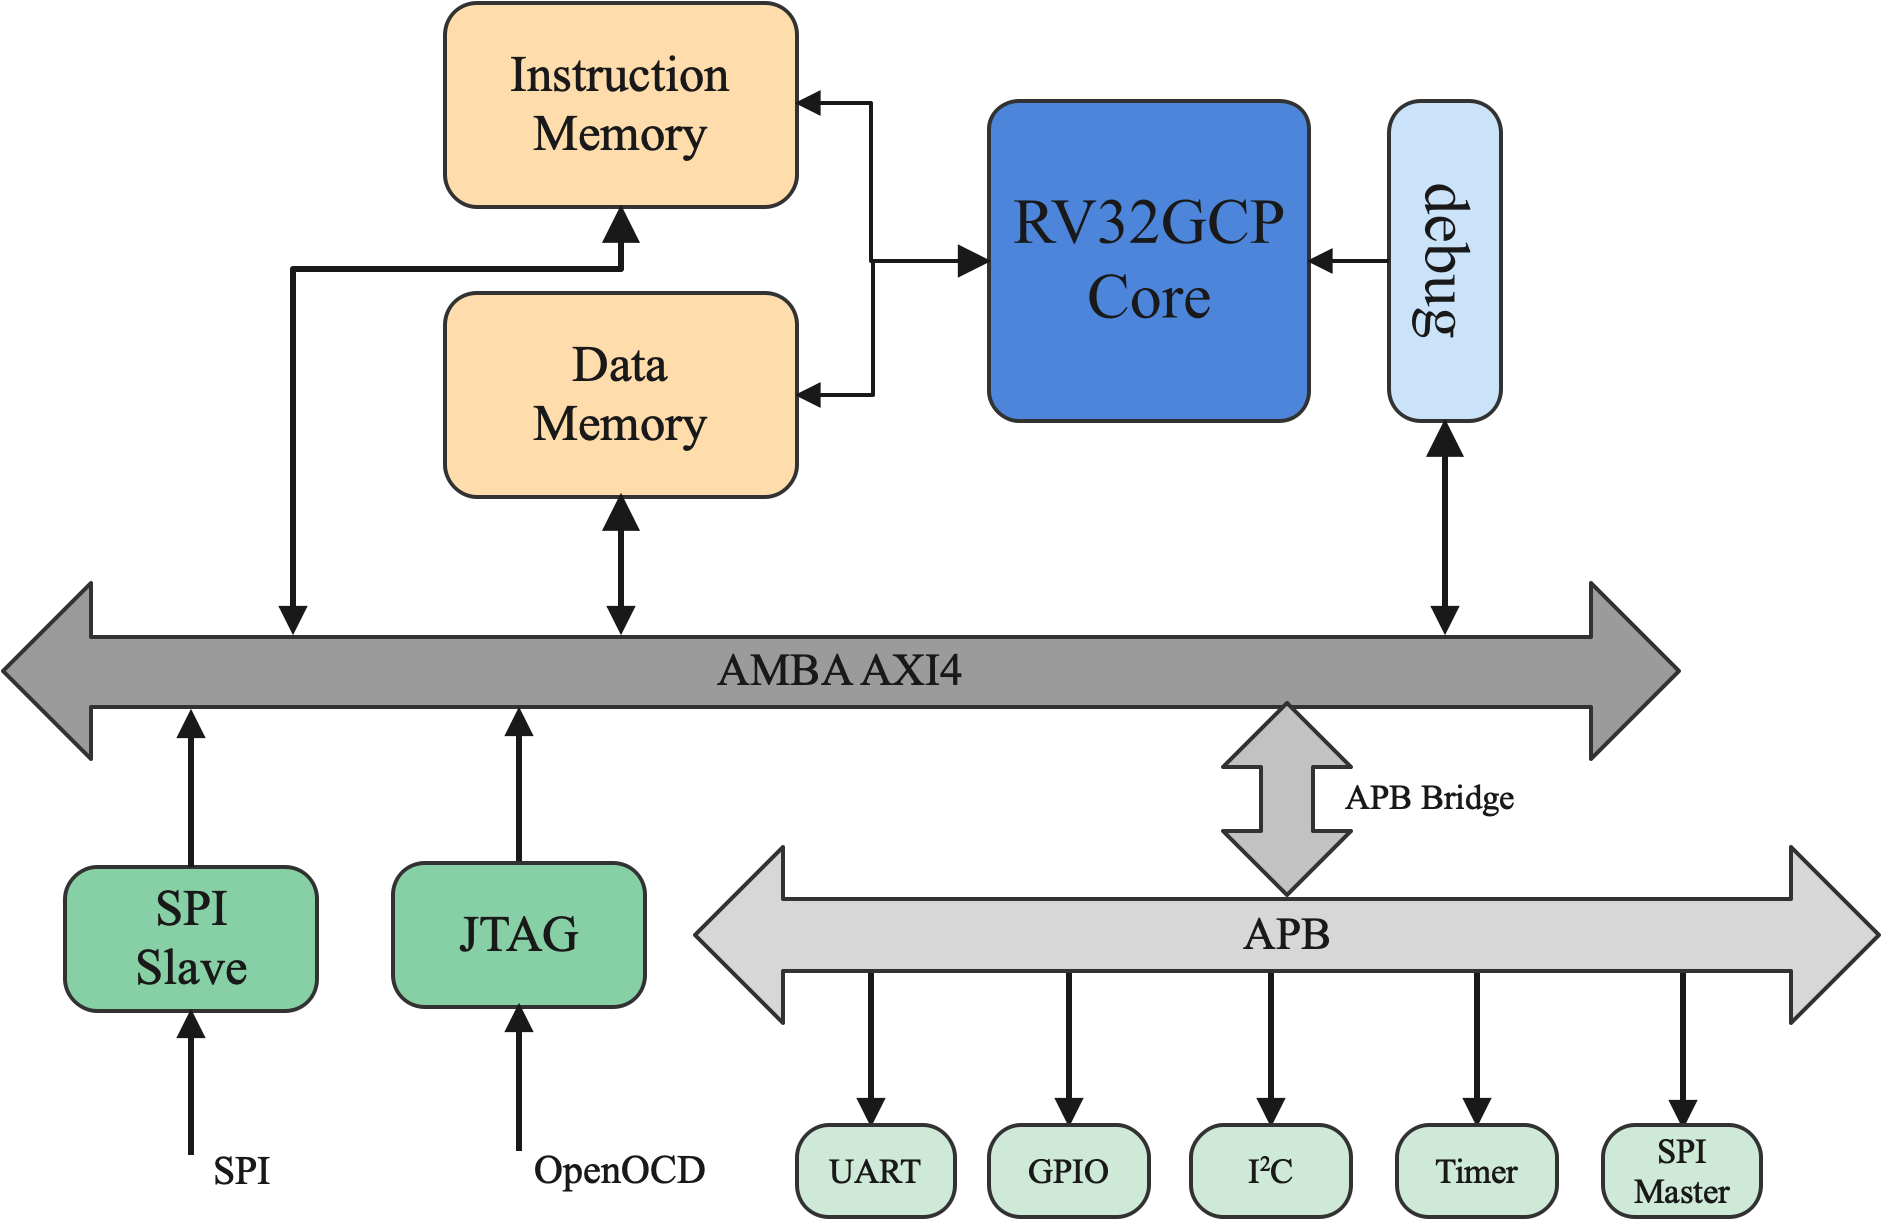
\includegraphics[width=0.95\textwidth]{Photos/SoC_Overview.png}
	\caption{包含RV32GCP RISC-V内核的SoC片上系统结构}
\end{figure}

\section{微处理器流水线细节}
\subsection{流水线概览}

基于性能以及功耗的综合考虑,本文的微处理器实现使用了单发射的顺序流水线结构,而非高性能微处理器中常用的顺序多发射超标量乱序执行处理器的结构。后者一般使用较为激进且复杂的分支预测策略以及托马苏洛算法[43]与重排序缓冲区来实现乱序执行,这种结构在性能上虽然比顺序发射执行的单发射流水线要好,但芯片整体的面积以及功耗无法达到嵌入式设备的需求。微处理器流水线的整体结构如图3-2所示。

\begin{figure}[htbp]
	\centering
	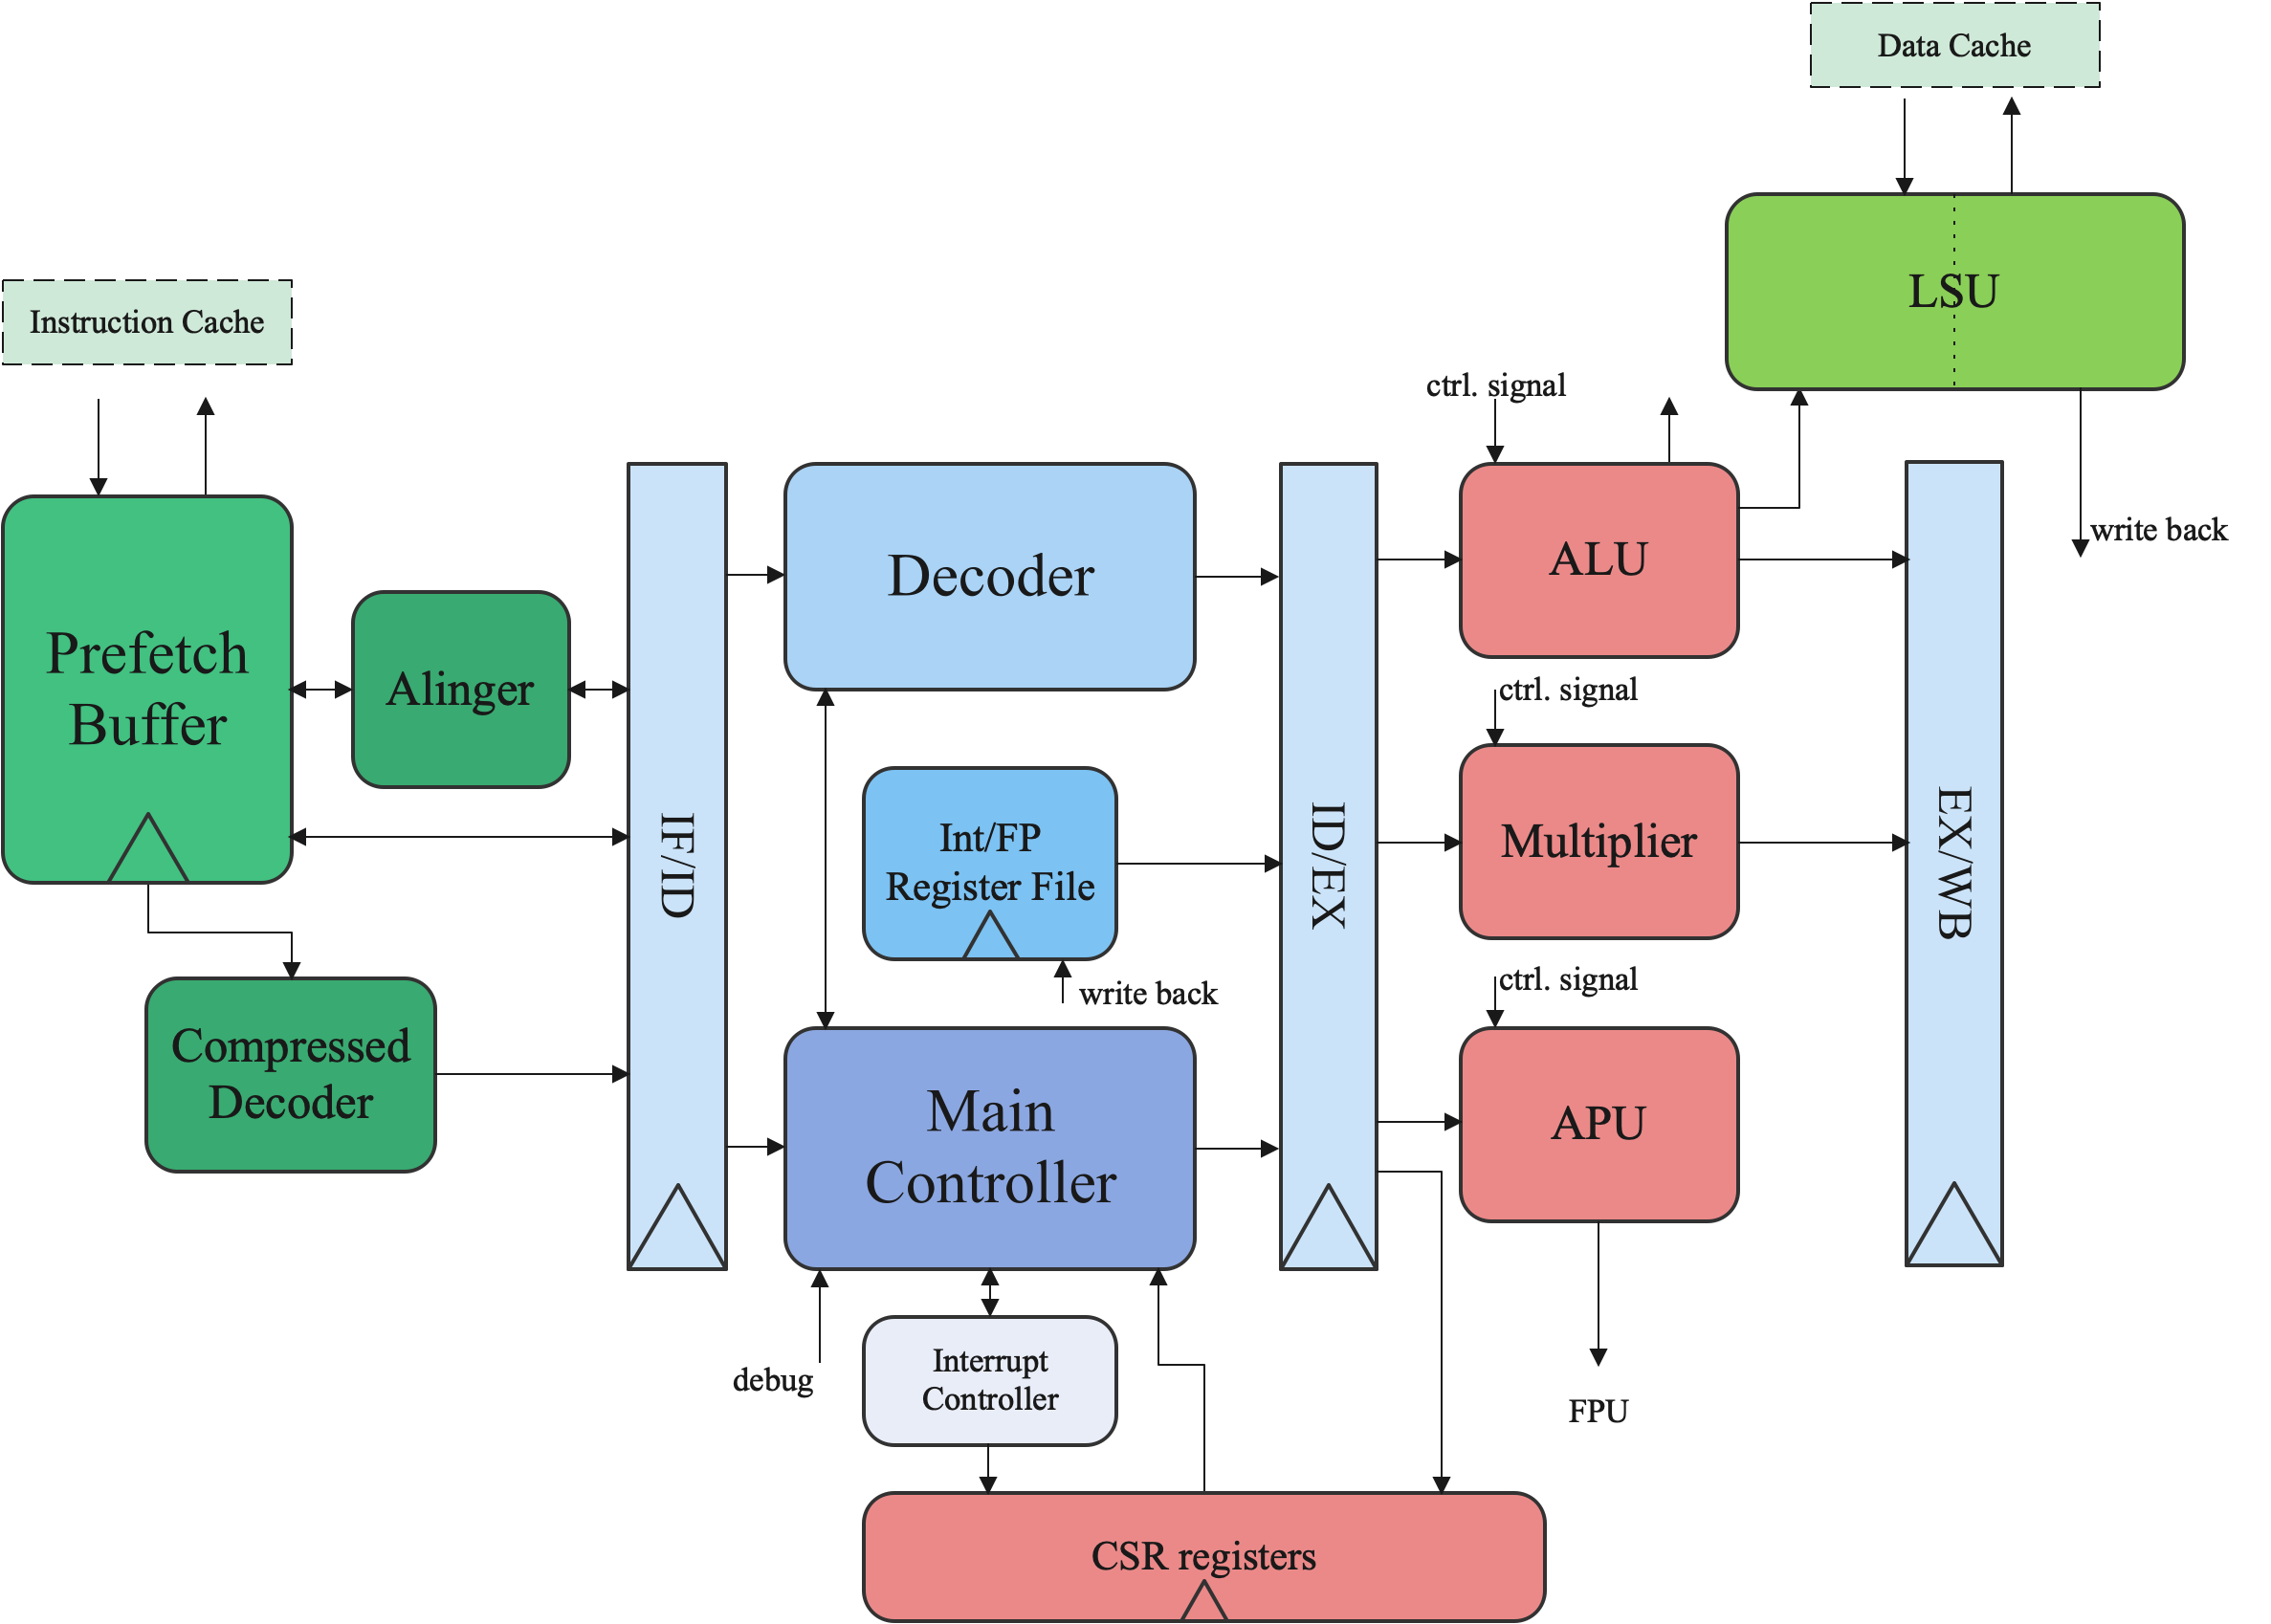
\includegraphics[width=0.95\textwidth]{Photos/Pipeline.png}
	\caption{微处理器流水线整体结构图}
\end{figure}

微处理器中4个流水线级的主要功能及作用概述:

\begin{enumerate}
	\item 取指阶段(Instruction Fetch,IF)。取指阶段通过核内自定义的总线协议(与LSU总线协议相同)从最低级的指令L1缓存中取指,并保存在一个小的预取缓冲区当中。预取缓冲区可以缓解因非对齐的指令地址所造成的停顿问题。同时取指阶段也会对16位的压缩指令进行预先的译码,转换为标准的32位RISC-V指令集传递到译码阶段。分支预测单元也包含在取指阶段当中。
	\item 译码阶段(Instruction Decode,ID)。译码阶段对取指阶段中的指令进行译码,并转化为若干控制信号控制微处理器中各功能单元的执行。译码阶段包含有译码器、主控制器以及中断控制器,其中无条件跳转指令在该阶段执行。
	\item 执行阶段(Execute,EX)。执行阶段包括执行指令所需要的功能单元:算术逻辑单元ALU、乘除法器以及协处理器接口单元APU。考虑到浮点运算功能实现的复杂度以及延迟,浮点功能通过APU与核外的浮点运算单元交互来实现。有条件跳转指令在该阶段执行,通过ALU对跳转条件进行判断,并将结果反馈到主控制器来控制是否进行分支。部分指令在执行阶段需要多个周期完成,对于多周期的指令,微处理器一律通过停顿来保证不会出现数据冒险。所有需要写回寄存器的算术逻辑指令在该阶段即完成写回操作。同时,针对存储器相关指令的地址也会在执行阶段生成,并传递给LSU。
	\item 写回阶段(Write back,WB)。写回阶段只对于加载指令有效,所有加载指令的写回在该阶段完成。这是因为通过自定义的总线协议从最低级的数据L1缓存中加载指令至少需要1个周期的时间才能返回数据。
\end{enumerate}

表3-1展示了微处理器中除浮点以及“P”扩展以外指令的周期数,所有执行周期大于1的指令都会导致流水线停顿并带来CPI(指令平均执行周期数,Cycle Per Instruction)的损失。

\begin{table}
	\caption{指令类型及其对应的执行周期数}
	\centering
	\small 
	\begin{tabular}{p{80pt}p{50pt}p{200pt}}
		\hline 
		指令类型 & 执行周期                & 备注             \tabularnewline
		\hline 
		RV32I 算术逻辑运算   & 1		     & 基本的RV32I算术逻辑运算只需要1个周期完成 \tabularnewline
		整数乘法   & 1或5	     & mul指令只需要1个周期,mulh、mulhsu、mulhu需要5个周期完成 \tabularnewline
		除法/取模   & 3到35	     & 除法与取模所需要的周期数取决于被除数前导零的个数 \tabularnewline
		无条件跳转   & 2     & 无条件跳转在ID阶段执行 \tabularnewline
		有条件跳转   & 1或3     & 不进行分支的有条件跳转不会带来停顿,进行分支的有条件跳转需要刷新IF及ID阶段。分支预测错误的跳转指令也需要3个执行周期。 \tabularnewline
		CSR访问   & 1或4     & 访问不同的控制状态寄存器需要不同的周期,具体定义在RISC-V的Zicsr指令集中 \tabularnewline
		加载/存储指令   & 1或2     & 对齐的加载/存储指令需要只需要1个周期,非对齐或者半字(16位)的加载/存储指令需要2个周期。 \tabularnewline
		\hline 
	\end{tabular}
\end{table}

微处理器实现中对冒险(Hazard)的处理如下:

\begin{enumerate}
	\item 对于结构冒险,由于多周期的指令一律通过流水线停顿处理,因此流水线中不存在同一周期中出现冲突的功能单元,不存在结构冒险。
	\item 对于数据冒险,由于流水线是顺序执行的,因此只存在写后读(RAW)冒险,不存在读后写(WAR)以及写后写(WAW)的数据冒险。对于写后读的数据冒险,主要通过旁路转发的方式进行处理,以尽可能的提高CPI。但仍存在两种情况需要停顿1个或多个周期来解决数据依赖:加载数据冒险,即紧跟在一条加载指令后的指令依赖于加载指令的目标寄存器数据;基于寄存器的链接跳转指令jalr的数据冒险,即一条jalr指令依赖于上一条指令的目标寄存器数据。
	\item 对于控制冒险,无条件跳转指令固定具有1个周期的惩罚,这是因为无条件跳转都在ID阶段执行,此时已经进入IF阶段的指令都会被刷新。有条件跳转取决于两个因素:是否执行分支以及分支预测是否正确。不执行的分支以及错误的分支预测都会导致已经进入IF、ID阶段的指令被冲刷掉,带来2个后期的惩罚。可以看出,有效的分支预测策略可以为CPI带来显著的提升。
\end{enumerate}

\subsection{取指阶段}

取指阶段将从最低级指令L1缓存中获取指令,并存储到预取缓冲区或直接传递给ID阶段,同时对压缩指令进行预先译码转换成32位标准指令传递给ID阶段。取指阶段还会对非对齐的指令地址访问进行处理。取指阶段的主要模块及其功能如下:

\begin{enumerate}
	\item 预取缓冲区:预取缓冲区可以实现对非对齐指令的单周期取指,以优化流水线的整体性能,其整体结构为一个先进先出的队列。
	\item 取指地址对齐单元:由于预取缓冲区请求的指令地址永远是32位对齐的,但本文实现的微处理器支持16位压缩指令,因此在指令L1缓存中混合有32位及16位的指令。取指地址对齐单元则用于处理非对齐指令读取的情况。
	\item 压缩指令译码器:将16位的RISC-V压缩指令译码为32位指令。
\end{enumerate}

预取缓冲区设计的主要目的是为了降低非对齐指令访问的延迟。如果不做任何处理,非对齐的指令访问需要2个时钟周期才能取得。预取缓冲区的默认大小为4个字节,即128位,可以保证在不占用过多面积的同时提升性能。下面以一个例子来说明预取缓冲区的设计如何实现非对齐指令的单周期取指。

如图3-3所示,假设当前PC指向地址为0x80的32位数据,其中低16位是压缩指令,而高16位是下一条32位指令的前16位。此时地址为0x84的32位数据已经被预取到预取缓冲区当中,因此首先将压缩指令传递到压缩指令译码器中译码并送至ID阶段,同时该32位的数据还会保存在取指地址对齐单元的寄存器中保留多一个时钟周期。下一个周期,PC指向变为0x84,则从预取缓冲区中直接读取下一个指令的高16位部分,并与上个周期的32位数据的高16位组成一个完整的指令传递给ID阶段,即可达到对非对齐的指令实行单周期读取的效果。如果没有预取缓冲区,则IF阶段需要发送非对齐的地址至指令L1缓存,指令L1缓存则需要分成2个周期来传送该指令,因此,预取缓冲区还可以使取指地址固定32位对齐,而不需要考虑压缩16位压缩指令与32位指令混合的情况。

\begin{figure}[htbp]
	\centering
	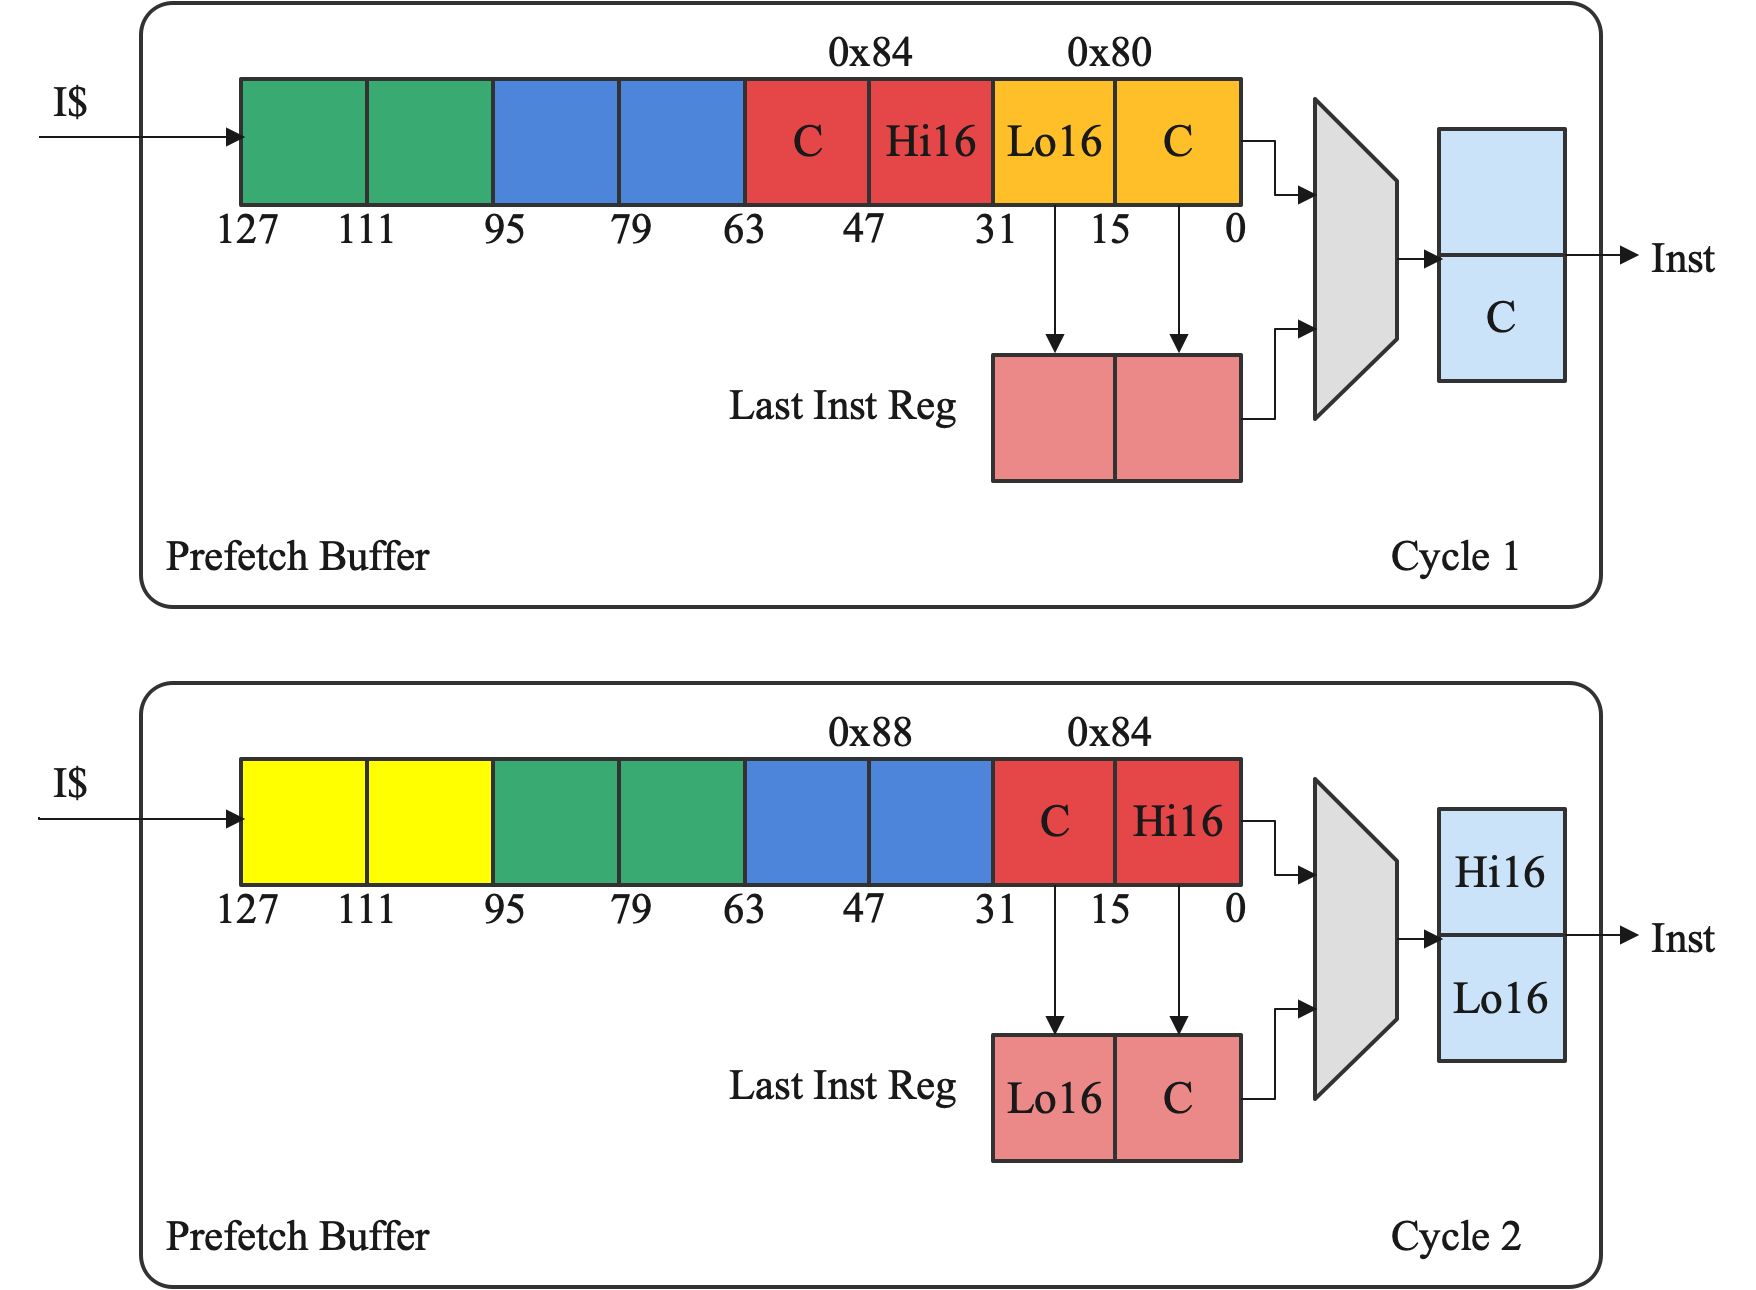
\includegraphics[width=0.95\textwidth]{Photos/PrefetchBuffer.png}
	\caption{单周期非对齐指令读取示例。其中“C”表示16位的RV32C指令,“Hi16”表示32位RISC-V指令的高16位,“Lo16”表示32位RISC-V指令的低16位。}
\end{figure}

取指地址对齐单元与预取缓冲区功能互相配合,其内部是一个状态机,状态机的状态主要取决于上一周期从对齐地址取回的32位数据及当前周期从对齐地址取回的32位数据内容情况,同时还要考虑当跳转指令目标地址也是非对齐情况时的处理,如跳转指令的目标地址也是一个16位的压缩指令。

压缩指令译码器是纯的组合逻辑结构,其功能仅简单的使用多个多路选择器将压缩指令译码为32位指令。

除此之外,取指阶段还包含有一个简单的分支预测器。分支预测器使用基于4K大小动态分支缓冲区的两位饱和计数器策略来预测分支是否执行,在保证面积优化的同时提高流水线的性能。对于目前较为流行的数种不同的分支策略,在权衡利弊后作出了如上选择,原因在于:

\begin{enumerate}
	\item 一个简单的使用4K项缓冲区全局二位饱和计数器分支预测策略在SPEC89测试上的预测准确率可以达到82\%到99\%,这种简单且空间较小的预测器所实现的动态分支预测策略相比于每次进行分支都冲刷IF、ID的流水线级间寄存器对CPI性能的提升要好。同时相比于静态的分支预测,该策略仅使用较小的缓冲区代价就可以带来相当高的性能改善。
	\item 高级的分支预测器如相关分支预测器[44, 45]、竞赛预测器[46]、带标记的混合预测器[47]具有相当高的分支预测准确率,在SPECint测试上最高可以达到97.8\%到98.2\%的分支预测准确率。但这些分支预测器的实现逻辑非常复杂,在面向低功耗的嵌入式系统当中实现并不现实。
\end{enumerate}

\subsection{译码阶段}

译码阶段将来自取指阶段的指令进行译码操作,并转换为若干控制信号发送给相关的执行单元执行当前指令。译码阶段还包括从整数寄存器组以及浮点数寄存器组的读取操作。中断控制器用于外部中断的仲裁及CSR寄存器组的交互。无条件跳转在译码阶段进行,将IF/ID流水线间寄存器冲刷,给流水线带来固定1个时钟周期的延迟。译码阶段的主要模块及其功能如下:

\begin{enumerate}
	\item 整数及浮点数寄存器组:带有32个32位整数寄存器以及32个32位浮点数寄存器的寄存器组模块。在本文的实现中基于FPGA的后端工艺采用了触发器的实现。寄存器组带有3个读端口以及2个写端口,以保证不会出现结构冒险的情况。整数寄存器以及浮点数寄存器共享相同的旁路以及写入的逻辑。
	\item 译码器:纯组合逻辑单元,将来自取指阶段指令译码并将相关信息传递到主控制单元。如果指令是无效的,将会触发内部异常。
	\item 主控制单元:接收来自译码器以及其他功能模块、流水线间寄存器的反馈信号,根据内部状态机的转移发出相应的控制信号到各功能模块。主控单元同时还负责接收来自外部的调试信号,以控制流水线的启停。
	\item 中断控制器:接收外部中断信号并基于中断优先级进行仲裁,将仲裁结果反馈到CSR寄存器组。若中断使能且有效,则跳转到相对应的中断服务程序。
\end{enumerate}

译码阶段的主要工作是根据RISC-V指令集标准对指令进行译码操作,其硬件逻辑主要是由大量多路选择器所组成的选择逻辑结构,在此不对这方面进行过多的赘述。

\subsection{执行阶段}

执行阶段接收来自译码阶段主控制器的控制信号,并根据信号执行指令。执行阶段最主要的功能模块为算术逻辑单元ALU,ALU负责执行RV32I中的基本整数算术逻辑运算以及“P”扩展指令集中的SIMD运算。乘除法的实现相互分离,除法器使用基本的串行移位除法器实现,整合在ALU当中。乘法器则作为单独的功能单元与ALU分离。执行阶段还包含一个辅助处理单元(Auxiliary Processing Unit,APU)来实现与流水线外部FPU单元交互。状态控制寄存器组(Control Status Registers,CSRs)也包含在执行单元,对CSR的读写操作在执行阶段进行。对于除存储器加载以外的指令来说,写回的操作也发生在执行阶段,换句话说,从执行阶段开始会对微处理器架构状态发生改变。执行阶段的主要模块及其功能如下:

\begin{enumerate}
	\item 算术逻辑单元ALU:ALU主要由以下的部分组成:一个32位整数加法器,由4个先行进位8位加法器组成、移位及比较单元、串行移位除法器、以及用于“P”扩展指令集中SIMD指令及其他指令的执行单元。有关“P”扩展指令的实现将在3.3节中进行叙述。
	\item 乘法器:乘法器包括一个32位乘32位的整数乘法器,对于非取结果高32位的指令(mulh系指令)只需要1个时钟周期即可完成,否则则需要5个时钟周期。32位的整数乘法器通过分区的方式实现,以此方便对“P”扩展指令集中SIMD指令的实现。
	\item 辅助处理单元:辅助处理单元通过自定义的接口协议与浮点处理单元(FPU)交互。与一般的总线协议类似,辅助处理单元在地址阶段发送浮点操作数、浮点操作以及请求信号至FPU,FPU运算后的结果在响应阶段发回到辅助处理单元。
	\item 控制状态寄存器组:CSRs包含一系列保存有微处理器当前状态信息的寄存器组,如机器模式状态寄存器mstatus,其中包含有当前微处理器所处的特权级模式、各特权模式下的中断使能状态等。与通用寄存器组不同,CSRs的读写需要一定的权限,如用户模式下尝试对机器模式的控制状态寄存器进行读写会引发内部异常。
\end{enumerate}

根据表3-1中所提到的,乘法器执行32位乘32位的整数乘法,在只需要低32位的结果时只需要1个时钟周期,而需要高32位的结果时则需要5个时钟周期。这是因为在只需要低32位的mul指令时,乘法器直接调用32位乘法器计算得到低32位结果。而在需要高32位的结果时,乘法器则使用分区的16位乘16位乘法,在5个时钟周期中分时计算并取高32位结果输出。在RTL级的代码实现中,一个简单的“*”运算符在进行逻辑综合时会根据乘法运算位数而生成不同大小以及复杂度的乘法器,因此需要谨慎考虑进行乘法运算时操作数的位数。逻辑综合器一般会对乘法器做一定的优化,如基于Radix-4的booth编码乘法器[48]、基于保留进位加法器的华莱士树等等,具体的优化策略根据综合时的约束综合器会生成不同的乘法器。

除法以及取模的运算需要最少3个时钟周期到35个时钟周期不等,这是因为除法器实现的是逻辑较为简单的串行移位除法器。除法器内部控制单元实现一个状态机,其中有3个固定的时钟周期用于启动以及结束运算,余下的为线性移位除法的运算周期。被除数的前导零越多,运算所需要的周期越少。与乘法不同,除法的优化空间不多,追求性能较高的除法器会牺牲大量的面积,因此在低功耗的微处理器实现中一般都使用较为简单的串行除法器。

外部FPU的设计采用参数化的设计方法,考虑到浮点运算的复杂性,FPU将浮点运算分为4大类来实现,分别为浮点加法与浮点乘法、浮点除法与浮点平方根、浮点比较、浮点与浮点/整数之间的转换。4大类运算使用并行的数据路径以及运算单元实现,且通过参数配置运算单元的流水级数。流水级数越少,运算所需要的时钟周期数越少,延时越低,但逻辑面积越大。

控制状态寄存器组的具体实现则遵循RISC-V特权级指令标准实现,在此不进行过多的赘述。

除此之外,还需要注意的一点是,在执行阶段ALU也会对存储器相关操作的地址进行运算并生成,提交到加载存储单元中,并向最低级数据L1级缓存发出请求。在下一个周期指令进入写回阶段,从缓存中读取的数据返回到LSU中,并写回到通用寄存器组。这就是为什么图16中LSU在结构上可以看作是横跨执行阶段以及写回阶段。

\subsection{写回阶段}

写回阶段主要是加载存储单元对从存储器读数据的阶段,即可以看作是内部总线协议的响应阶段。只有从存储器中加载数据到通用寄存器组的指令才会到达写回阶段。指令处于写回阶段的时间取决于存储器的延时。为了提高流水线的效率,LSU以及自定义的内部总线协议允许多个存储器的请求同时进行,并按照顺序返回。如果存储器延时较大,即需要多个时钟周期才能返回读取数据,则为了避免数据冒险,需要流水线停顿响应的周期直到所需要的数据从存储器中读取返回到LSU当中。

\section{微处理器特权模式及异常中断处理机制实现}

本文所实现的微处理器仅实现了RISC-V特权级模式标准中的机器模式,这是考虑到本微处理器的应用场景主要是低功耗的嵌入式系统,在此类系统中一般只需要少量的任务调度以及资源分配,且中断处理时间是此类系统中微处理器时间中显著的一部分。RISC-V特权级模式标准中没有对外部中断的仲裁以及优先级做出规定,因此在外部中断的仲裁以及中断优先级的分配方面需要自己实现。本微处理器实现了CLINT实现对外部中断以及内部异常的仲裁与控制。

CLINT实现一共有32个中断,优先级从31号到0号中断自高到低排列。其中高16个中断是用户自定义的外部中断。低16个中断则是预留给核内的软件以及计时中断等,需要注意的是硬件计时中断拥有所有中断中的最高优先级,这是中断号按优先级顺序中的例外。当有多个中断等待服务时,则根据中断优先级依次进行处理。

微处理器中包含有3种核内异常:非法指令、断点以及ECALL(机器模式下的执行环境调用指令)。异常的优先级总是高于中断,需要立即进行处理。异常与中断的主要区别在于,异常处理返回的地址是出现异常的指令地址或下一条指令的地址,而中断处理返回的地址则是中断响应时指令的下一条指令地址。

下面给出本文所实现微处理器对异常以及中断的处理流程:

首先,若当前所需要处理的是中断,则当中断使能时,则进入该中断。异常无法屏蔽,处理器必须立刻处理异常。进入异常或者中断后,微处理器中的行为:

\begin{enumerate}

\item 更新机器模式异常程序计数器mepc。mepc是一个32位可读写的CSR,如果出现的是中断,则将当前执行的指令的下一条指令地址写入到mepc中。如果出现的是一场,则将当前指令地址写入到mepc中。
\item 更新机器模式异常原因寄存器mcause。微处理器根据异常产生的原因更新mcause。如果是中断,则户籍将mcause中的中断位置1。
\item 更新机器模式异常值寄存器mtval。mtval中保存有异常相关的信息,如当一个硬件的断点触发,或者指令的获取,或者加载存储地址未对齐,或者页故障异常发生时,mtval会写入受异常影响的地址。在非法指令的异常当中,mtval会写入故障指令。对于其他的异常来说,mtval会写入为0。
\item 更新机器模式状态寄存器mstatus。将异常或中断发生前的机器模式中断全局使能位MIE保存到机器模式中断全局使能位保留栈MPIE当中,将异常或中断发生前所处的特权级保存到机器模式特权级保留栈MPP中,在本微处理器实现下恒为机器模式。将MIE设为0。在特权级标准中,RISC-V是不支持嵌套中断的[49]。若要实现嵌套中断,则只能通过软件的方式来实现。具体实现:当一个异常发生后,则MPIE设置为MIE的值,MIE设为0,同时MPP设置为机器模式。本微处理器实现同样仅支持软件的中断嵌套。
\item 跳转到机器模式异常入口基地址寄存器mtvec中所定义的异常入口地址执行。mtvec有两种模式,一种是直接模式,直接跳转到mtvec中的基地址执行。另一种是向量模式,根据mcause中的异常类型跳转到对应的异常处理程序首地址中执行。

\end{enumerate}

当异常或中断处理程序执行完毕后,在程序最后会调用MRET指令来退出异常处理程序(其他特权级的指令为SRET、URET,本微处理器实现不需要)。执行MRET指令后微处理器硬件执行的行为如下:


\begin{enumerate}
\item 从mepc中定义的地址执行。恢复到异常或中断发生前的程序流执行。
\item 更新mstatus。将异常发生前的mstatus的状态恢复,具体实现:此时MIE从MPIE中恢复,特权模式设置为M,MPIE设置为1,MPP设置为M。
\end{enumerate}

至此异常或中断的处理结束,微处理器回到触发异常或者中断的指令或者下一条指令继续执行。

\section{"P"扩展指令集的实现}

“P”扩展指令集是RISC-V为了增强对数字信号处理相关算法的运算性能所提出的扩展指令集。“P”扩展指令集可以使支持的RISC-V微处理器能够在低功耗的前提下对DSP相关应用保持较高的处理性能。“P”扩展指令集总共有3大类的指令:SIMD数据处理指令、部分SIMD数据处理指令(主要是乘后加MAC指令)以及少量的非SIMD指令。

SIMD数据处理指令主要包括8位以及16位的加减法、移位、比较以及乘法指令,部分SIMD指令主要包括不同位宽的乘后加MAC指令,非SIMD指令主要包括不同位宽的饱和运算(Saturation Arithmetic)。同时处理的数据量由当前微处理器的字长决定。如果当前微处理器的字长为32位,则8位的SIMD指令则同时处理4个8位数据。换句话来说,“P”扩展指令集的SIMD指令主要通过将与当前微处理器字长相同的寄存器中的数据划分为若干相同位宽的数据同时进行运算。这是“P”扩展指令集与“V”向量扩展指令集最大的区别。“P“扩展指令集中的SIMD实现方式较为简单,所有指令的位宽都是固定的,但缺乏一定的灵活性。而”V“向量扩展指令集则通过向量专用CSR寄存器来配置向量大小、向量中元素的位宽来动态改变同时执行运算的元素数量及位宽大小。”V“扩展的实现适合高性能的图像处理或者深度学习应用,但会带来相当大的功耗以及面积。因此本微处理器采用了更为低功耗的”P“扩展指令进行实现。

“P”扩展指令集主要通过扩展译码器以及ALU来实现,通过参数配置来决定是否生成”P“扩展指令的相关逻辑。下面将通过一个例子来说明微处理器实现“P”扩展指令中SIMD指令的主要思路。以8位加法的SIMD指令“ADD8”为例子,该指令的操作如下所示:

\begin{equation}
rd.B[x] = rs1.B[x] + rs2.B[x]
\end{equation}

其中B[x]代表源操作数寄存器以及目标寄存器中的第x个字节。在本文所实现的32位微处理器中,x的取值是0到3。也就是说,该指令将同时将寄存器rs1中的4个单子节数据**同时**与rs2中的4个单子节数据相加,并将结果写入到寄存器rd中对应的字节当中。在“P”指令集中,所有的SIMD指令的基准是微处理器的字长,也就是单个寄存器的位宽,因此在实现的时候可以重用基于RV32GC实现的数据路径而不需要做出改变,只需要在译码器以及ALU当中做相应的扩展。而“V”向量扩展指令则是通过向量CSR寄存器中的值来决定当前向量的长度以及元素位宽,为了构成相应长度的向量,可能需要将多个通用寄存器进行拼接,因此需要重新设计整个流水线的数据通路。

回到ADD8指令的实现上,根据如上所述,该指令可以重用在“P”扩展指令集实现前的数据通路,则该指令主要实现的关键点在于ALU。在3.1.4节中提到,ALU中为RV32I基本的加法指令实现的32位整数加法器中,是通过4个8位先行进位加法器实现的,这是为了兼容“P”扩展指令集而设计,如图3-4所示,在进入ALU前,从两个源操作数寄存器中读取的32位数据作为整体传递到ALU当中,ALU接收到控制器的控制信号,判定当前执行的是“ADD8”的SIMD指令,通过多路选择将4个先行进位加法器中对下一个加法器的进位置零,就可以实现同时对4个8位整数的同时相加。同时,在2.1节中提到的PyHCL函数式编程特性,在实现SIMD相关的运算操作时可以使用高阶函数大幅简化电路逻辑的表达过程。

\begin{figure}[htbp]
	\centering
	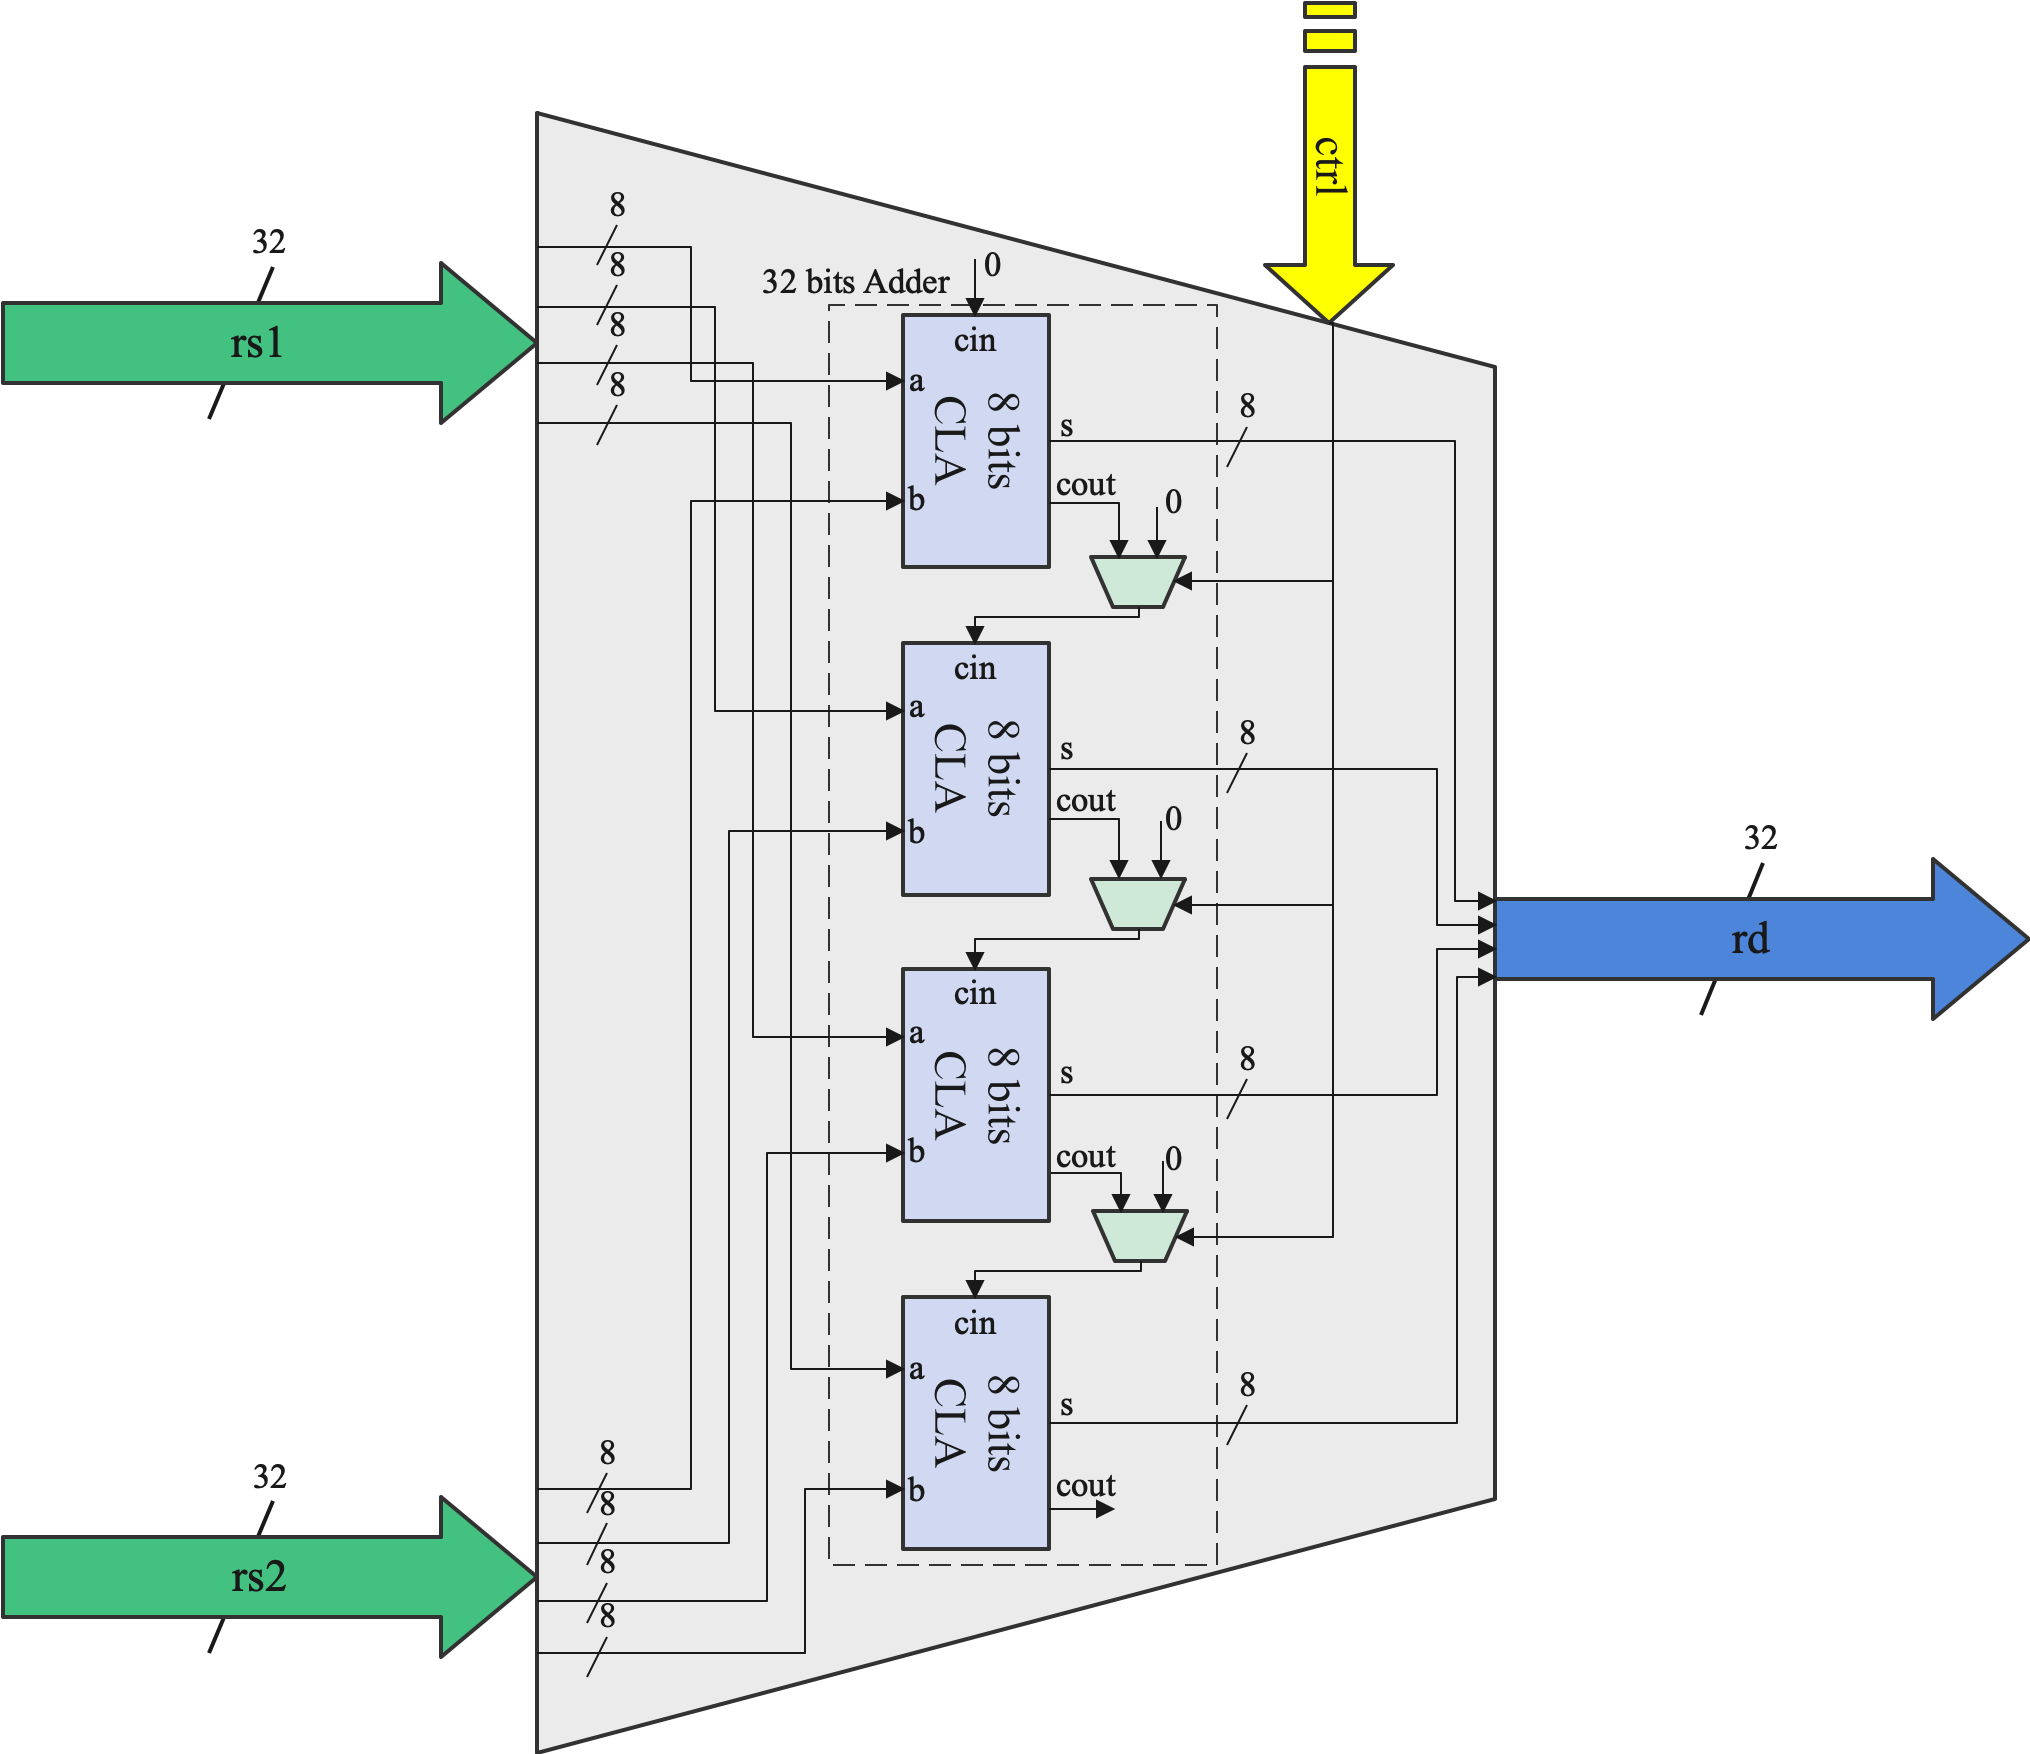
\includegraphics[width=0.95\textwidth]{Photos/ADD8.png}
	\caption{ALU中能够同时执行基本RV32I 32位加减法运算以及“P”扩展指令的SIMD加减运算的32位分区加法器。其中分割为4个8位的先行进位加法器。}
\end{figure}

\section{SoC实现以及相关测试数据}

在本章开头图13给出了包含本文实现的微处理器软核的SoC系统结构概览。SoC使用AMBA AXI4总线来作为内部的高速互联总线,而对于低速的外围设备,如UART、I2C等外设,则使用较为简单的APB总线。AXI4总线与APB总线之间通过APB桥交互。存储器方面,由于SoC进行测试的目标后端为FPGA平台,因此指令以及数据的存储器使用FPGA内置的BRAM资源构成,指令以及数据存储的大小为32K字节。SoC中还包含有一块大小为512字节的Boot ROM,存放启动系统的RISC-V汇编代码。SoC平台同时包含一个支持JTAG的调试器,可以在上位机通过OpenOCD进行GDB调试。调试器、数据及指令存储器通过AXI4总线进行互联。

表4列出了SoC片上系统中存储器以及外设在微处理器中的内存映射地址范围。SoC上电启动后,微处理器的PC启动地址为0x00080000,从Boot ROM中执行相关的配置指令,之后跳转到指令存储器中开始执行程序流。

\begin{table}
	\caption{SoC内存映射地址}
	\centering
	\small 
	\begin{tabular}{ccc}
		\hline 
		用途 & 大小                & 地址范围             \tabularnewline
		\hline 
		指令存储   & 32KB		     & 0x0000 0000 - 0x0000 7FFF \tabularnewline
		Boot ROM   & 512B		     & 0x0008 0000 - 0x0008 01FF \tabularnewline
		数据存储   & 32KB		     & 0x0010 0000 - 0x0010 7FFF \tabularnewline
		外设   & 32KB		     & 0X1A10 0000 - 0X1A10 7FFF \tabularnewline
		调试器   & 4KB		     & 0x1A11 0000 - 0x1A11 0FFF \tabularnewline
		\hline 
	\end{tabular}
\end{table}

其中,32KB的指令存储中0x00000000到0x0000008C地址范围预留为中断向量表,SoC外设使用自定义的16个外部中断与内核交互。

<相关数据>

\section{本章小结}

本章对本文使用PyHCL实现的基于RISC-V的RV32GCP微处理器进行的介绍,对微处理器的流水线、特权级模式以及异常与中断的实现机制、“P”扩展指令集的实现思路以及SoC片上系统进行具体的描述。本文所实现的微处理器在保持低功耗的目标前提下尽可能的考虑性能上的优化,通过使用简单而有效基于4K缓冲区的两位饱和计数分支预测器、紧凑的预取指缓冲区、分区的加法器以及乘法器等设计,以在追求资源与面积最优化的同时,提高微处理器的性能表现。本章的最后给出了包含该微处理器核的SoC片上系统在Xilinx N4 FPGA平台上的各项测试数据。